%%%%%%%%%%%%%%%%%%%%%%%%%
% !TEX TS-program = pdflatex
% !TEX root = ../tesis.tex
%%%%%%%%%%%%%%%%%%%%%%
%% CHAPTER 4
%%%%%%%%%%%%%%%%%%%%%%

%%%%%%%%%%%%%%%%%%%%%%%%%
\chapter{Application of ...}\label{chap_04}
%%%%%%%%%%%%%%%%%%%%%%%%%
\minitoc
% Define the algorithm per chapter (it has to be put in each chapter where one is put in).
\setcounter{algocf}{0} % Reset the algorithm counter in each chapter
\renewcommand{\thealgocf}{\thechapter.\arabic{algocf}} % Numbering of algorithms by chapters

\vspace{1cm}


\section{Introduction}

Lorem ipsum dolor sit amet, consectetur adipiscing elit. Sed do eiusmod tempor incididunt ut labore et dolore magna aliqua. Ut enim ad minim veniam, quis nostrud exercitation ullamco laboris nisi ut aliquip ex ea commodo consequat.



\section{Methodology}

Lorem ipsum dolor sit amet, consectetur adipiscing elit. Sed do eiusmod tempor incididunt ut labore et dolore magna aliqua. Ut enim ad minim veniam, quis nostrud exercitation ullamco laboris nisi ut aliquip ex ea commodo consequat.


\section{Results}

This is a placeholder paragraph intended to demonstrate the layout and formatting of the text. The actual content will be written here once the structure of the thesis is defined and the main arguments are developed accordingly.

Figure~\ref{fig:regions} illustrates...

\begin{figure}[!h]
  \centering
 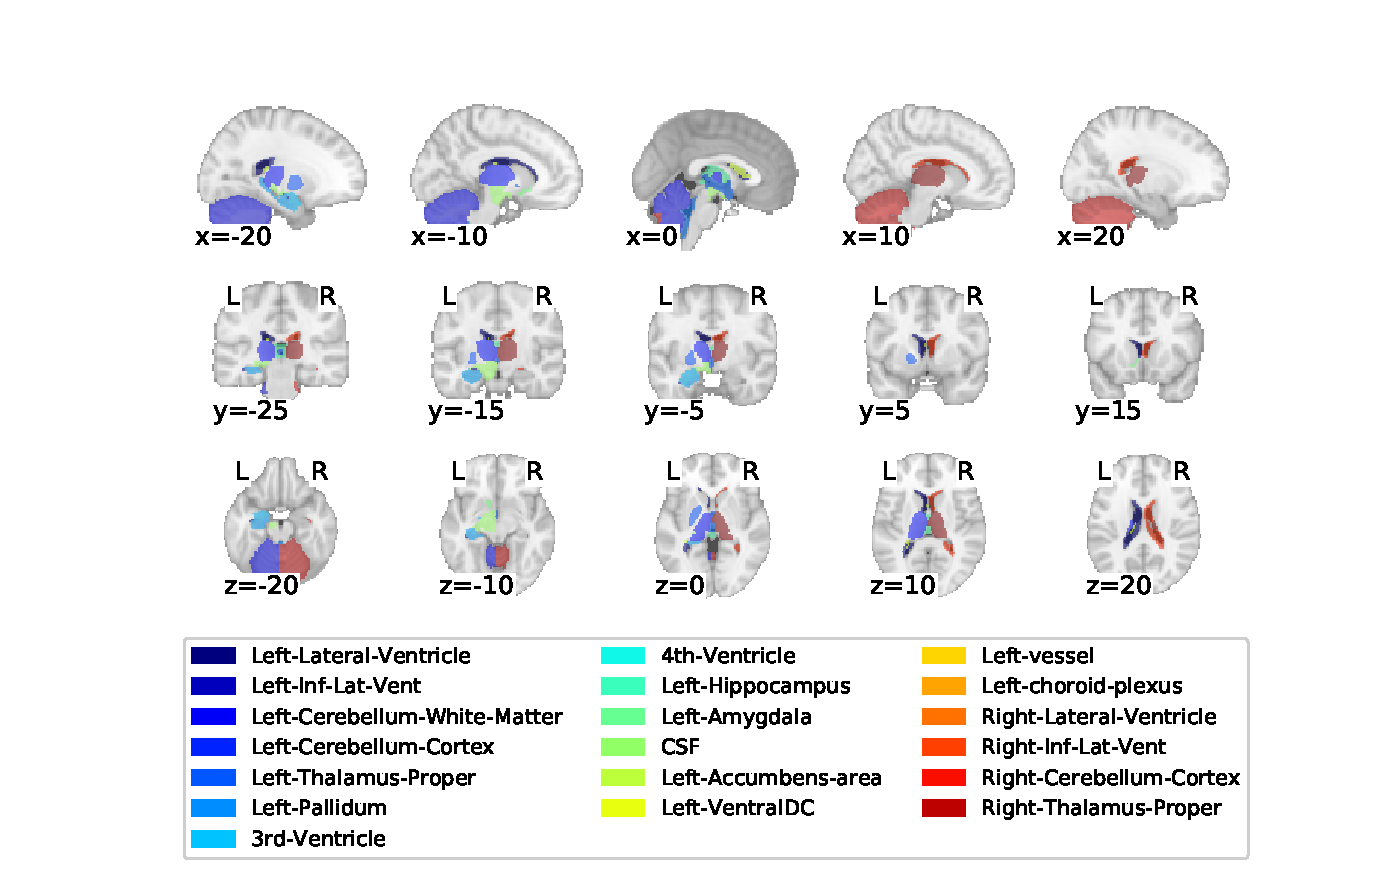
\includegraphics[width=0.7\textwidth]{Figures/chap_04/ROI7}
\caption{Selected regions after one-vs-one $t$-test feature selection.}\label{fig:regions}
\end{figure}

Table~\ref{tab:all} summarises ...

\begin{table}[htb]
\centering
\resizebox{0.8\textwidth}{!}{ \begin{tabular}{ccccccccc}
\toprule
\multicolumn{2}{l}{ }    & \multicolumn{3}{l}{\textbf{Training}}   &     & \multicolumn{3}{l}{ \textbf{Test (without dummies)}}  \\
\textbf{Ensemble} & \textbf{Classifier}  & Accuracy & Recall &F1-score & & Accuracy & Recall &F1-score \\
\midrule
-& SVM lineal              & 0.48     & 0.47   & 0.47   & & \textbf{0.67}   & \textbf{0.52}     & \textbf{0.66} \\
-& SVM RBF                 & 0.47     & 0.47   & 0.48   & &  0.67   & 0.52  & 0.63 \\
LogitBoost& Decision Tree & 0.48  & 0.44   & 0.51   &  & 0.64   & 0.46     & 0.60 \\
Random forest&Decision Tree & 0.48     & 0.44   & 0.52 & & 0.64   & 0.51     & 0.57 \\
AdaBoost&Decision Tree   & 0.50     & 0.42   & 0.47  &  & 0.60   & 0.43     & 0.52 \\
-&                  $5$-NN & 0.52     & 0.43   & 0.44  &  & 0.60   & 0.44     & 0.46 \\
-&                   $1$-NN & 0.52     & 0.39  & 0.42  & &  0.58   & 0.39     & 0.44 \\
-&                  $3$-NN & 0.51     & 0.40   & 0.39  & &  0.58   & 0.41     & 0.40 \\
-&                   MLP & 0.56     & 0.57   & 0.56  & &  0.60   & 0.60    & 0.59 \\
-&                   \acs{CNN} & 0.55     & 0.55  & 0.54  & &  0.48   & 0.47     & 0.48 \\
\bottomrule
 \multicolumn{6}{@{}l}{{\letratabla NN stands for nearest neighbours.}}
\end{tabular}}
\caption{Performance results for selected features using different classifiers.}\label{tab:all}
\end{table}


\section{Discussion}

Lorem ipsum dolor sit amet, consectetur adipiscing elit. Sed do eiusmod tempor incididunt ut labore et dolore magna aliqua. Ut enim ad minim veniam, quis nostrud exercitation ullamco laboris nisi ut aliquip ex ea commodo consequat.
